%versi 2 (8-10-2016)
\chapter{Landasan Teori}
\label{chap:teori}


Pada bab ini akan berisi landasan-landasan teori yang dipakai pada penelitian ini.

\section{Code Igniter}
\label{sec:codeigniter}


CodeIgniter\cite{codeigniter3} adalah \textit{framework} untuk pembuat website yang menggunakan \textit{PHP}. \textit{CodeIgniter} mempermudah \textit{developer} untuk meminimalisir penggunaan kode untuk mengakses suatu fungsi. Seperti untuk mengambil data pada \textit{database}, mengakses file \textit{php} lainnya. Penggunaan \textit{framework CodeIgniter} juga mudah.\textit{ Developer} tidak perlu melakukan banyak konfigurasi--konfigurasi saat melakukan \textit{setup}.\textit{CodeIgniter} juga memberikan dokumentasi yang lengkap. Permasalahan \textit{routing}  sudah diselesaikan oleh \textit{framework} ini. \textit{ Framework} ini secara otomatis akan mengarah ke file dalam \textit{directory controllers} sesuai dengan \textit{path-abempty} pada \textit{URI}  dan menjalankan \textit{method} \codefont{index()}.


\begin{figure}[H]
	\centering
	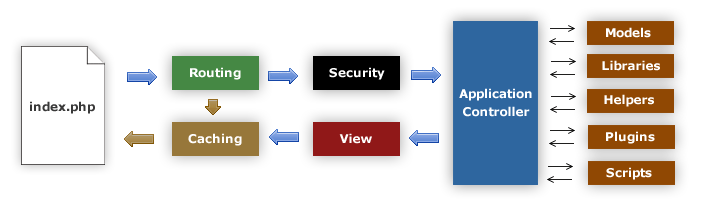
\includegraphics[scale=0.8]{mvc} 
	\caption{Flowchart MVC}
	\label{fig:appflowchart} 
\end{figure}


\textit{CodeIgniter} menerapkan arsitektur \textit{MVC} yang dapat dilihat pada gambar \ref{fig:appflowchart}, file \codefont{index.php} berfungsi mengatur routing dan mengarahkan ke \textit{application controller} yang berada di \textit{directory controller} dan melalui \textit{controller} akan dipanggil \textit{models, libraries, helpers, etc} yang dibutuhkan dengan perintah \codefont{\$this->load-><<apa\_yang\_mau\_diload>>(\lq<<nama\_file>>\rq)}. Masukan akan diolah melalui \textit{models} dan hasil yang sudah siap akan dikirim ke \textit{view} melalui \textit{controller}. Fitur tambahan dari arsitektur \textit{CodeIgniter} adalah saat \textit{router} memeriksa \textit{HTTP request} jika \textit{cache} tersedia maka akan dikirimkan \textit{cache} tersebut dan jika tidak ada \textit{cache} maka \textit{security} akan memeriksa dan melakukan filter terhadap \textit{HTTP request} seperti pada gambar \ref{fig:appflowchart}. 

\subsection{Controller}

\textit{Controller} adalah pusat dari aplikasi, \textit{controller} menangani apa yang harus dilakukan dari \textit{HTTP request}. Dalam CodeIgniter untuk menginisiasi \textit{controller} cukup menulis nama kelas diikuti dengan \codefont{extends CI\_Controller} sebagai contoh:

\begin{table}[H]
\begin{lstlisting}
<?php
defined('BASEPATH') OR exit('No direct script access allowed');
		
class Welcome extends CI_Controller {

	public function index()
	{
		$this->load->view('welcome_message');
	}
}
\end{lstlisting}
\end{table}
\smallskip

\textit{CodeIgniter} secara otomatis akan menjalankan \textit{method} \codefont{index()} jika tidak diperintahkan untuk menjalankan \textit{method} tertentu. Untuk menjalankan \textit{method} lain hanya perlu ditambahkan \textit{path-abempty} seperti  \codefont{example.com/index.php/Welcome/<<nama\_method>>}.
fungsi diatas akan mengembalikan file \textit{welcome\_message.php} pada direktori \textit{view}. Developer dapat menaruh parameter pada \textit{view} tersebut.

\smallskip
\begin{table}[H]
\begin{lstlisting}
<?php
defined('BASEPATH') OR exit('No direct script access allowed');
	
class Welcome extends CI_Controller {
	
	public function __construct(){
		parent::_construct();
		$this->load->database();
		$this->load->model(contoh_model);
	}
	
	public function index()
	{
		$t = "hello";
		$this->load->view('welcome_message',array(
		't' => $t));
	}
}
\end{lstlisting}
\end{table}
\smallskip
Fungsi \textit{constructor} yang dijalankan pada \textit{codeigniter} harus memanggil \codefont{parent::construct()}. Dalam contoh diatas juga dapat dilakukan \textit{load model} dan \textit{database}. File \textit{model} akan berada di direktori \textit{model} sedangkan untuk \codefont{\$this->load->database()} akan melakukan \textit{load} pada \textit{database} menggunakan parameter yang ada di direktori \codefont{/config/database.php}. Begitu juga dengan kebutuhan--kebutuhan lainnya dapat dilakukan dengan \textit{method} \codefont{\$this->load}.


\subsection{Model}

\textit{Model} berfungsi sebagai \textit{logic} dari aplikasi. \textit{ Model} pada \textit{CodeIgniter} bersifat opsional, tetapi disediakan untuk \textit{developer} yang ingin menggunakan MVC\cite{codeigniter3}. 

\begin{table}[H]
\begin{lstlisting}
class Blog_model extends CI_Model {

	public $title;
	public $content;
	public $date;
	
	public function get_last_ten_entries()
	{
		$query = $this->db->get('entries', 10);
		return $query->result();
	}
}
\end{lstlisting}
\end{table}

\textit{Model} pada \textit{CodeIgniter} harus diikuti dengan \codefont{extends CI\_MODEL}. Hal yang berurusan terhadap \textit{database} dapat dilakukan dengan perintah \codefont{\$this->db->query(\lq<<isi query>>\rq)} atau untuk mempermudah, beberapa fungsi \textit{MYSQL} dasar disediakan oleh \textit{CodeIgniter}.\textit{ Method} bisa langsung digunakan seperti \codefont{\$this->db->get(\lq<<nama tabel>>\rq)}
untuk mengambil semua nilai dari tabel tersebut. Untuk dapat mengakses \textit{database} maka harus dipasang \textit{database} yang akan digunakan pada \codefont{config/database.php}.
\begin{table}[H]
\begin{lstlisting}
		
$config['hostname'] = 'localhost';
$config['username'] = 'myusername';
$config['password'] = 'mypassword';
$config['database'] = 'mydatabase';
$config['dbdriver'] = 'mysqli';
$config['dbprefix'] = '';
$config['pconnect'] = FALSE;
$config['db_debug'] = TRUE;

$this->load->model('model_name', '', $config);
\end{lstlisting}
\end{table}

File \codefont{database.php} diatas menyimpan kredensial dari \textit{database} yang digunakan. Mulai dari \textit{hostname, username, password, dst}.

\subsection{View}


\textit{View} tidak pernah dipanggil secara langsung, \textit{view} harus dipanggil melalui \textit{controller}\cite{codeigniter3}.
\textit{View} pada \textit{CodeIgniter} ditaruh pada direktori \textit{view}. Pemanggilan \textit{view} menggunakan \textit{method} 
\begin{lstlisting}
$this->load->view('nama_view');
\end{lstlisting}
Jika \textit{controller} ingin mengirimkan data kepada \textit{view} maka perlu dilakukan 
\begin{lstlisting}
$t = "hello";
$this->load->view('welcome_message',array(
't' => $t));
\end{lstlisting}
Selanjutnya untuk menampilkan data tersebut ke halaman 
\begin{lstlisting}
html>
<head>
</head>
<body>
	<h1><?php echo $t ?></h1>
</body>
</html>
\end{lstlisting}




\section{Phpspreadsheet}
\label{section:phpspreadsheet}

\begin{table}[H]
	\centering
	\begin{tabular}{|p{0.5\textwidth}|c|c|}
		\hline
		\textbf{Format} & \textbf{Reading} & \textbf{Writing} \\ \hline
		Open Document Format/OASIS (.ods) & \checkmark & \checkmark \\ \hline
		Office Open XML (.xlsx) Excel 2007 and above & \checkmark & \checkmark \\ \hline
		BIFF 8 (.xls) Excel 97 and above & \checkmark & \checkmark \\ \hline
		BIFF 5 (.xls) Excel 95 & \checkmark  & \\ \hline
		SpreadsheetML (.xml) Excel 2003 & \checkmark & \\ \hline
		Gnumeric & \checkmark & \\ \hline
		HTML & \checkmark & \checkmark \\ \hline
		SYLK & \checkmark & \\ \hline
		CSV & \checkmark & \checkmark \\ \hline
		PDF (using either the TCPDF, Dompdf or mPDF libraries, which need to be installed separately) & & \checkmark \\ 
		\hline
	\end{tabular}
\caption{Tabel format yang didukung oleh phpspreadsheet}
\label{tab:phpspreadsheet supported}
\end{table}


PhpSpreadsheet adalah \textit{library} yang ditulis dengan bahasa PHP berguna untuk membaca dan menulis file dengan jenis spreadsheet seperti Excel dan LibreOffice Calc\cite{phpspreadsheet}. Format--format yang didukung oleh phpspreadsheet dapat dilihat pada tabel \ref{tab:phpspreadsheet supported}. Pada penelitian kali ini phpspreadsheet hanya digunakan untuk menulis ke dokumen dengan \textit{extension} \codefont{.xls}

\subsection{Instalasi Phpspreadsheet}
Sebelum dapat menginstalasi phpspreadsheet dibutuhkan composer. Composer dapat diunduh pada \url{getcomposer.org}. dan menjalankan perintah:

\begin{lstlisting}
composer require phpoffice/phpspreadsheet
\end{lstlisting}
Masukkan perintah tersebut untuk membuat file \codefont{composer.json} dan menginstalasi \textit{dependencies} tersebut. Contoh untuk menggunakan phpspreadsheet dapat dilihat sebagai berikut:

\begin{lstlisting}
<?php

require 'vendor/autoload.php';

use PhpOffice\PhpSpreadsheet\Spreadsheet;

$spreadsheet = new Spreadsheet();
$sheet = $spreadsheet->getActiveSheet();
\end{lstlisting}

Kode diatas akan membuat spreadsheet dengan isi \lq Hello World !\rq pada kolom A1. Penggunaan phpspreadsheet secara dasar dibutuhkan perintah \codefont{use PhpOffice$\backslash$PhpSpreadsheet$\backslash$Spreadsheet} dan \codefont{new Spreadsheet()}.

\subsection{Menempatkan Nilai pada Kolom tertentu}

\subsection{Menulis Spreadsheet ke Xls }

\section{Bootstrap}


\section{\LaTeX}
\label{sec:latex}

Mengapa menggunakan \LaTeX{} untuk buku skripsi dan apa keunggulan/kerugiannya bagi mahasiswa dan pembuat template. 

\dtext{13-14}


\section{Template Skripsi FTIS UNPAR}
\label{sec:template}
 
Akan dipaparkan bagaimana menggunakan template ini, termasuk petunjuk singkat membuat referensi, gambar dan tabel.
Juga hal-hal lain yang belum terpikir sampai saat ini. 
 
\dtext{15-16}

\subsection{Tabel}  
Berikut adalah contoh pembuatan tabel. 
Penempatan tabel dan gambar secara umum diatur secara otomatis oleh \LaTeX{}, perhatikan contoh di file bab2.tex untuk melihat bagaimana cara memaksa tabel ditempatkan sesuai keinginan kita.

Perhatikan bawa berbeda dengan penempatan judul gambar gambar, keterangan tabel harus diletakkan di atas tabel!!
Lihat Tabel~\ref{tab:contoh1} berikut ini:

\begin{table}[H] %atau h saja untuk "kira kira di sini"
	\centering 
	\caption{Tabel contoh}
	\label{tab:contoh1}
	\begin{tabular}{cccc}
		\toprule
		& $v_{start}$ & $\mathcal{S}_{1}$ & $v_{end}$\\

		\midrule
		$\tau_{1}$ & 1 & 12& 20\\
		$\tau_{2}$ & 1 &  & 20\\
		$\tau_{3}$ & 1 & 9 & 20\\
		$\tau_{4}$ & 1 &  & 20\\

		\bottomrule
		
	\end{tabular} 
\end{table}
Tabel~\ref{tab:cthwarna1} dan Tabel~\ref{tab:cthwarna2} berikut ini adalah tabel dengan sel yang berwarna dan ada dua tabel yang bersebelahan. 
\begin{table}[H]
	\begin{minipage}[c]{0.49\linewidth}
		\centering
		\caption{Tabel bewarna(1)}
		\label{tab:cthwarna1}
		\begin{tabular}{ccccc}
			\toprule
			 & $v_{start}$ & $\mathcal{S}_{2}$ & $\mathcal{S}_{1}$ & $v_{end}$\\
			
			\midrule
			$\tau_{1}$ & 1 & 5 \cellcolor{green}& 12& 20\\
			$\tau_{2}$ & 1 & 8 \cellcolor{green}& & 20\\
			$\tau_{3}$ & 1 & 2/8/17 \cellcolor{green}& 9 & 20\\
			$\tau_{4}$ & 1 & \cellcolor{red}& & 20\\
			
			\bottomrule

		\end{tabular}
	\end{minipage}
	\begin{minipage}[c]{0.49\linewidth}
		
		\centering 
		\caption{Tabel bewarna(2)}
		\label{tab:cthwarna2}
		\begin{tabular}{ccccc}
			\toprule
			 & $v_{start}$ & $\mathcal{S}_{1}$ & $\mathcal{S}_{2}$ & $v_{end}$\\
			
			\midrule
			$\tau_{1}$ & 1 & 12& 5 \cellcolor{red} &20\\
			$\tau_{2}$ & 1 &  &  8 \cellcolor{green} &20\\
			$\tau_{3}$ & 1 & 9 & 2/8/17 \cellcolor{green} &20\\
			$\tau_{4}$ & 1 &   & \cellcolor{red} &20\\
			
			\bottomrule
		
		\end{tabular}
	\end{minipage}
\end{table}

 
\subsection{Kutipan}
\label{subs:kutipan} 
Berikut contoh kutipan dari berbagai sumber, untuk keterangan lebih lengkap, silahkan membaca file referensi.bib yang disediakan juga di template ini.
Contoh kutipan:
\begin{itemize}
	\item Buku:~\cite{berg:08:compgeom} 
	\item Bab dalam buku:~\cite{kreveld:04:GIS}
	\item Artikel dari Jurnal:~\cite{buchin:13:median}
	\item Artikel dari prosiding seminar/konferensi:~\cite{kreveld:11:median}
	\item Skripsi/Thesis/Disertasi:~\cite{lionov:02:animasi}~\cite{wiratma:10:following}~\cite{wiratma:22:later}
	\item Technical/Scientific Report:~\cite{kreveld:07:watertight}
	\item RFC (Request For Comments):~\cite{RFC1654}
	\item Technical Documentation/Technical Manual:~\cite{Z.500}~\cite{unicode:16:stdv9}~\cite{google:16:and7}
	\item Paten:~\cite{webb:12:comm}
	\item Tidak dipublikasikan:~\cite{wiratma:09:median}~\cite{lionov:11:cpoly}
	\item Laman web:~\cite{erickson:03:cgmodel}  
	\item Lain-lain:~\cite{agung:12:tango}
\end{itemize}    
  
\subsection{Gambar}

Pada hampir semua editor, penempatan gambar di dalam dokumen \LaTeX{} tidak dapat dilakukan melalui proses {\it drag and drop}.
Perhatikan contoh pada file bab2.tex untuk melihat bagaimana cara menempatkan gambar.
Beberapa hal yang harus diperhatikan pada saat menempatkan gambar:
\begin{itemize}
	\item Setiap gambar {\bf harus} diacu di dalam teks (gunakan {\it field} {\sc label})
	\item {\it Field} {\sc caption} digunakan untuk teks pengantar pada gambar. Terdapat dua bagian yaitu yang ada di antara tanda $[$ dan $]$ dan yang ada di antara tanda $\{$ dan $\}$. Yang pertama akan muncul di Daftar Gambar, sedangkan yang kedua akan muncul di teks pengantar gambar. Untuk skripsi ini, samakan isi keduanya.
	\item Jenis file yang dapat digunakan sebagai gambar cukup banyak, tetapi yang paling populer adalah tipe {\sc png} (lihat Gambar~\ref{fig:ularpng}), tipe {\sc jpg} (Gambar~\ref{fig:ularjpg}) dan tipe {\sc pdf} (Gambar~\ref{fig:ularpdf})
	\item Besarnya gambar dapat diatur dengan {\it field} {\sc scale}.
	\item Penempatan gambar diatur menggunakan {\it placement specifier} (di antara tanda  $[$ dan $]$ setelah deklarasi gambar.
	Yang umum digunakan adalah {\bf H} untuk menempatkan gambar {\bf sesuai} penempatannya di file .tex atau  {\bf h} yang berarti "kira-kira" di sini. \\
	Jika tidak menggunakan {\it placement specifier}, \LaTeX{} akan menempatkan gambar secara otomatis untuk menghindari bagian kosong pada dokumen anda.
	Walaupun cara ini sangat mudah, hindarkan terjadinya penempatan dua gambar secara berurutan. 	
	\begin{itemize}
		\item Gambar~\ref{fig:ularpng} ditempatkan di bagian atas halaman, walaupun penempatannya dilakukan setelah penulisan 3 paragraf setelah penjelasan ini.
		\item Gambar~\ref{fig:ularjpg} dengan skala 0.5 ditempatkan di antara dua buah paragraf. Perhatikan penulisannya di dalam file bab2.tex!
		\item Gambar~\ref{fig:ularpdf} ditempatkan menggunakan {\it specifier} {\bf h}.
	\end{itemize}
\end{itemize}
 
\dtext{17-18}
\begin{figure} 
	\centering  
	\includegraphics[scale=1]{ular-png}  
	\caption[Gambar {\it Serpentes} dalam format png]{Gambar {\it Serpentes} dalam format png} 
	\label{fig:ularpng} 
\end{figure} 

\dtext{19-20}
\begin{figure}[H]
	\centering  
	\includegraphics[scale=0.5]{ular-jpg}  
	\caption[Ular kecil]{Ular kecil} 
	\label{fig:ularjpg} 
\end{figure} 
\dtext{21-22}

\begin{figure}[ht] 
	\centering  
	\includegraphics[scale=1]{ular-pdf}  
	\caption[ {\it Serpentes} betina]{ {\it Serpentes} jantan} 
	\label{fig:ularpdf} 
\end{figure} 
 
